\section{数据预处理与可视化}

\subsection{数据介绍}

本实验的数据来源于Mathlib4开源项目\cite{mathlib4},该项目是一个数学证明库,其中包含了大量的数学定理和证明。在Mathlib4中,相关的数学定理和证明被组织成了单个lean4文件,每个lean4文件中包含了一个或多个数学定理和证明。在本实验中,我们将lean4文件看作是一个节点,节点之间的依赖关系看作是一条有向边,这样我们就可以将Mathlib4中的数学定理和证明组织成一个有向图。

\subsection{数据预处理}

Mathlib4中不仅有数学定理的证明,还包括一些lean4的库文件、编译脚本、证明策略等等。在本实验中,我们筛选出了数学定理和证明,而去除了其他文件。然后进行依赖的提取。

为了快速地得到Mathlib4中数学概念的大致依赖关系,我们把每个lean4文件中直接使用import关键字引入的其他lean4文件看作是该文件的一个依赖,而没有使用编译器前端或者lsp等进行依赖分析。但实际上,由于lean4灵活的命名空间,lean4文件之间的依赖关系可能会比我们所统计的要复杂。另一方面,单个lean4文件也可能包含相当多的数学定理和证明,这具体取决于代码贡献者是否严格遵循Mathlib4的编程规范以及仓库管理者是否对代码贡献者的代码进行了严格地审核。因此,我们的数据只能作为Mathlib4中数学定理和证明的一个大致依赖关系的参考。

按照上面的方法,我们把Mathlib4中的文件的依赖关系提取出来之后,共有4910个节点和13858条边,我们把数据保存为一个json文件,以便之后使用。

\subsection{数据可视化}

把上文中提取出的数据进行可视化,我们可以得到Mathlib4中各个学科的依赖图。图中的每个节点代表一个lean4文件,节点之间的边代表依赖关系,节点的颜色取决于其所在的子学科,边的颜色与被依赖的节点相同。下图\ref{fig:dependency}展示了Mathlib4中的各个子学科的依赖关系。

\begin{figure}[H]
    \centering
    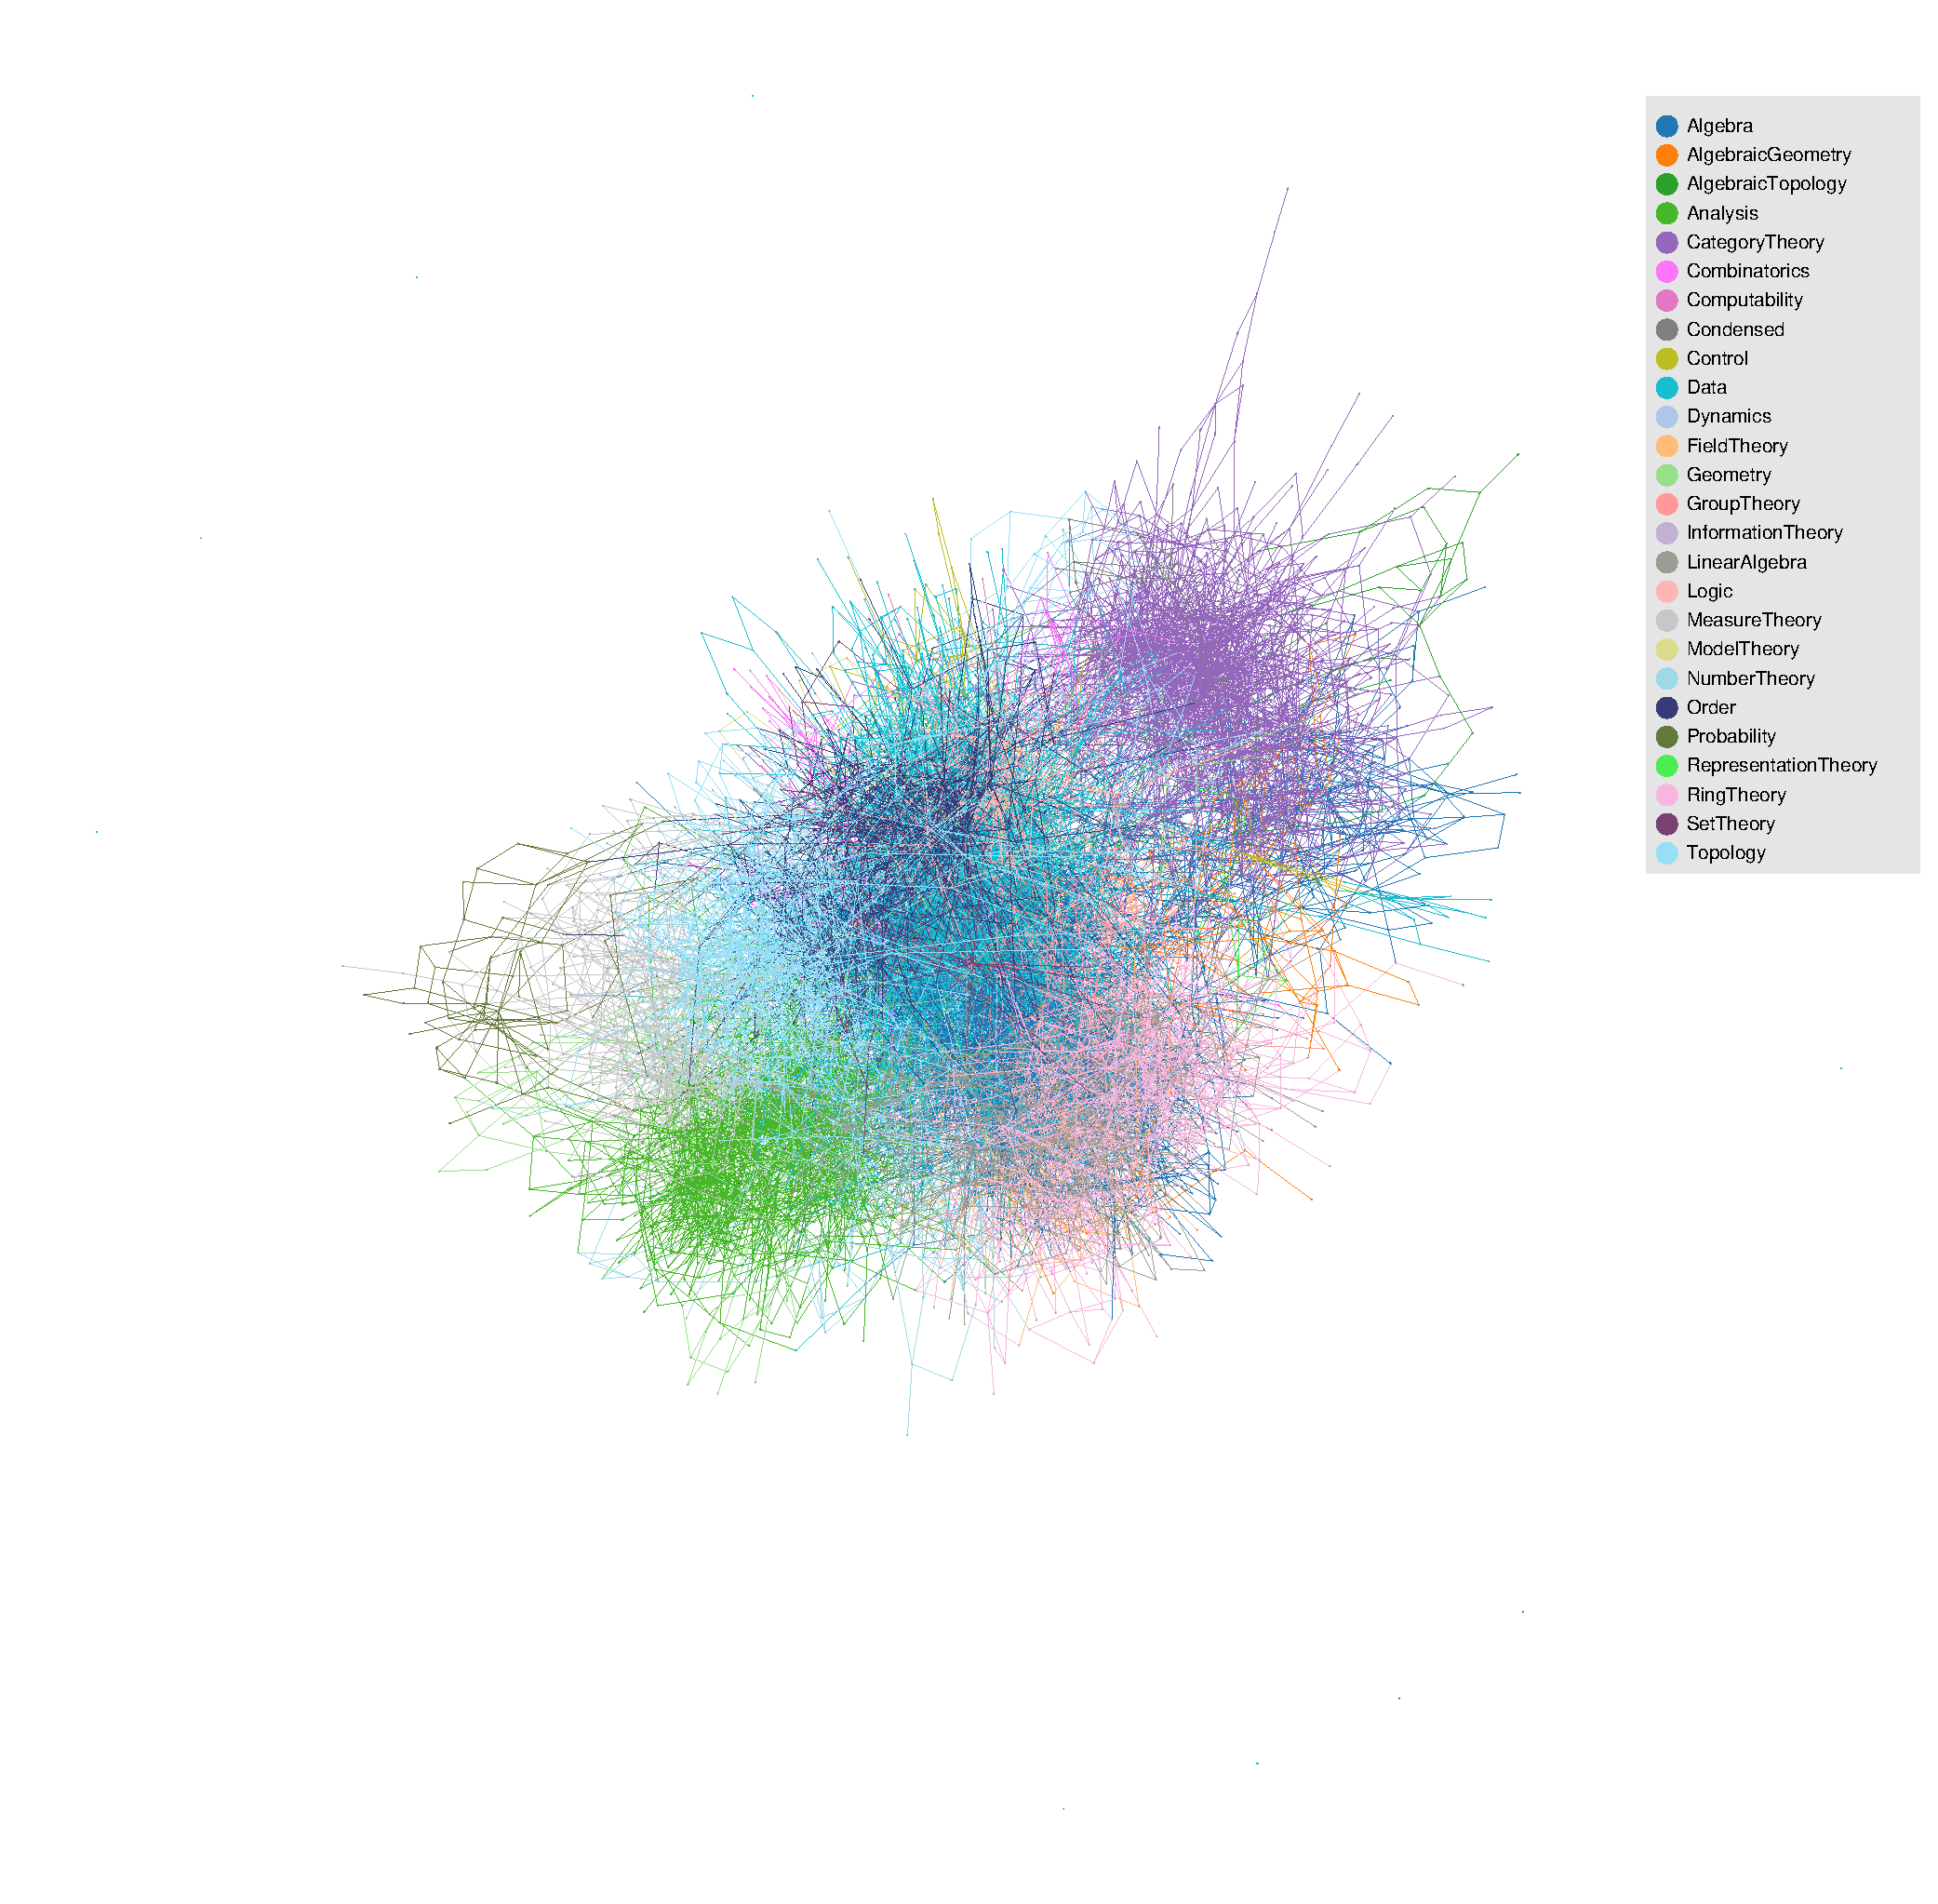
\includegraphics[width=1.0\textwidth]{../img/graph_new.png}
    \caption{Dependency graph of Mathlib4}
    \label{fig:dependency}
\end{figure}

如上图\ref{fig:dependency}所示,我们确实可以图中有明显的各色团簇,这说明该图中存在一定的社群结构,尽管可能这个社群结构并不一定与其按学科划分的社群完全一致。
